The central diagnostic of Phase I is an information-loss ladder.
Consider what the environment provides and what the persistent variables
of the substrate can possibly retain. Figure~\ref{fig:ladder}
schematizes the cascade; each rung is a compression the substrate
performs automatically, and each was measured where the instruments
allowed.

\paragraph{Rung 1: afferent structure.}
Patterns are channel groups; the persistent synaptic structure develops
selectivity for them (selectivity \(\pm 0.8\)--\(0.9\),
\S\ref{sec:organization}). At this rung, structure exists and survives
silence.

\paragraph{Rung 2: instantaneous spikes.}
At any instant, the internally observed quantity is the spike train.
Spikes carry the full timing information of the stimulus, but they are
activity: the substrate does not store them.

\paragraph{Rung 3: windowed counts.}
The measured representation of a presentation is its 500 ms spike-count
vector. This is the rung at which the organization is assayed
(response separation) and it is stimulus-locked: off-window
(count-free) responses do not separate. The architectural review
measured during-window cross-pattern separation cosines 0.30--0.89 but
off-window 0.999+, and the V2.2-era and E21 records fixed the temporal
carry of the substrate below 50 ms (gap-0 retention only:
\(D_{L{-}NF}=0.0815\)) \cite{overview}.

\paragraph{Rung 4: cumulative counts.}
The substrate has one integrator that accumulates over presentations:
the slow state \(u\) (V2.1), \(u \mathrel{+}= \beta\) per spike with
decay \(\tau_s\). Under drive it saturates to a flux balance (W1 cell:
mean \(u \to \approx 1.32\) by presentation \(\sim\)30). The
integration is over \emph{the organism's own spiking}, which under
drive is stimulus-locked but conflates patterns through the shared
pool (\S\ref{sec:organization}).

\paragraph{Rung 5: intrinsic scalar \(u\).}
What survives into silence is the integrated scalar field. Its
information content is the subject of §\ref{sec:u}: it is a population
rate trace, not a sensory memory.

\subsection{The dilution result across repeated presentations}

The loss that matters for persistent learning is not between rungs 1
and 2 but in what \emph{repeated} presentations do to episode identity
at the persistent rungs. The alternating-regime measurements
\cite{synmem} provide the sharpest quantitative statement: after each
presentation, the state of the synaptic store after an \(A\)
presentation and the state after the adjacent \(C\) presentation
converge --- the cosine of the per-neuron A-mass vector after \(C_k\)
versus after \(A_k\) rises \(0.972 \to 0.990\) over
\(k = 1 \to 40\). Simultaneously the alternating store becomes a
\emph{third configuration}, not a mixture of the trained endpoints
(cosine to the A-only endpoint 0.277, to the C-only endpoint 0.235,
while the endpoints are at 0.119 from each other; the best linear
mixture leaves 96\% of the alternating norm as residual)
\cite{synmem}. In other words: with alternation, episode identity is
diluted to a superposition; with blocking, it is overwritten
(§\ref{sec:interference}); at the persistent rungs the store converges
to quantities that cannot answer ``which episode, most recently.''

The same convergence was first measured in \(u\) (alternating-\(u\)
cosine \(\to 1.0\)) and then reproduced at the synaptic level --- the
records emphasize that the superposition failure is a property of the
shared additive store, not of the particular substrate
\cite{synmem}. Figure~\ref{fig:dilution} plots the two measured faces
of the dilution: the converging adjacent-state cosine (left) and the
within-block response-count decay (right), from the preserved
alternating and blocked runs respectively.

\begin{quote}
\textbf{Demonstrated:} the persistent storage rungs (synaptic weights;
integrated \(u\)) do not retain episode identity under repeated or
alternated exposure; adjacent-episode state similarity rises toward
1 (0.972 \(\to\) 0.990).\\[1pt]
\textbf{Supported:} the loss occurs at the transition from
presentation-local (spikes, counts) to persistent (integrals, weights)
representations; the shared-budget additive store is the mechanism
(later confirmed by the CLLA-era results, §\ref{sec:clla}).\\[1pt]
\textbf{Not established:} any persistent rung that distinguishes recent
episodes --- this is the negative result that motivates the rest of the
paper.
\end{quote}

\begin{figure}[t]
\centering
\resizebox{\textwidth}{!}{%
% Figure 3 — the information-loss ladder (schematic with measured annotations).
\begin{tikzpicture}[
  rung/.style={draw, rounded corners=2pt, minimum width=3.4cm,
               minimum height=9mm, align=center, font=\small},
  arr/.style={-{Stealth[length=2mm]}, thick}
]
  \node[rung, fill=green!8]  (r1) at (0, 0)   {afferent structure\\\footnotesize persistent, selective};
  \node[rung, fill=gray!8]   (r2) at (0, -1.3) {instantaneous spikes\\\footnotesize activity, not stored};
  \node[rung, fill=gray!8]   (r3) at (0, -2.6) {windowed counts\\\footnotesize stimulus-locked};
  \node[rung, fill=gray!8]   (r4) at (0, -3.9) {cumulative counts\\\footnotesize $u$: +$\beta$/spike, $\tau_s$};
  \node[rung, fill=red!8]    (r5) at (0, -5.2) {intrinsic scalar $u$\\\footnotesize persistent, info-poor};
  \draw[arr] (r1) -- (r2); \draw[arr] (r2) -- (r3);
  \draw[arr] (r3) -- (r4); \draw[arr] (r4) -- (r5);
  % measured annotations
  \node[font=\footnotesize, align=left, text width=6.3cm] (a1) at (4.6, 0.35)
    {selectivity $\pm0.8$--$0.9$,\\91\% run-identity decode \cite{synmem}};
  \node[font=\footnotesize, align=left, text width=6.3cm] (a3) at (4.6, -2.25)
    {off-window cosine $\ge 0.999$;\\temporal carry $< 50$ ms (E21)};
  \node[font=\footnotesize, align=left, text width=6.3cm] (a4) at (4.6, -3.55)
    {$\bar u$ saturates $\to 1.32$ under drive;\\alternating-$u$ cosine $\to 1$};
  \node[font=\footnotesize, align=left, text width=6.3cm] (a5) at (4.6, -4.9)
    {Fano $\approx 0$; pacemaker core (5--6 neurons);\\Gini 0.80 $\to$ 0.93 \cite{infoaudit}};
  \node[font=\footnotesize, align=left, text width=6.3cm] (a2) at (4.6, -0.95)
    {within-class $0.97$--$0.99$ across S1 halves;\\cross-class $0.70$--$0.81$ \cite{e1proto}};
\end{tikzpicture}
}
\caption{\textbf{The persistent-state information bottleneck.}
The substrate's automatic compression cascade: afferent structure
(persistent, selective) \(\to\) instantaneous spikes (activity)
\(\to\) windowed counts (stimulus-locked, not retained) \(\to\)
cumulative counts (the slow integrator \(u\)) \(\to\) intrinsic scalar
\(u\) (persistent but information-poor; §\ref{sec:u}). Each arrow is a
lossy compression performed by the substrate's own dynamics.}
\label{fig:ladder}
\end{figure}

\begin{figure}[t]
\centering
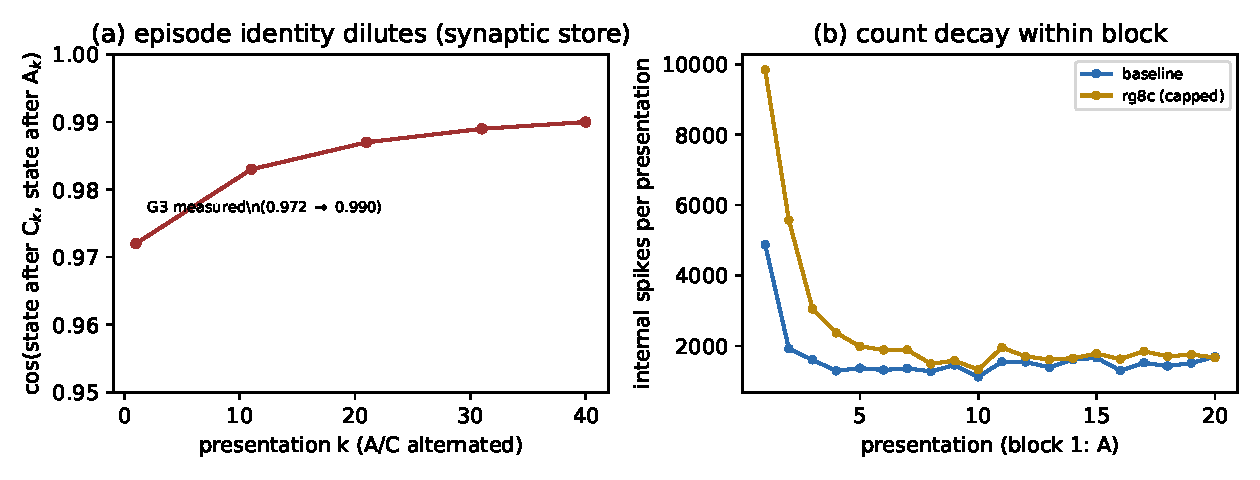
\includegraphics[width=\linewidth]{figures/fig4-dilution.pdf}
\caption{\textbf{Information dilution across repeated presentations.}
Left: convergence of the synaptic store after adjacent \(A\) and \(C\)
presentations under alternation (cosine 0.972 \(\to\) 0.990;
\cite{synmem}). Right: per-presentation internal spike counts decay
within a blocked block (baseline run), the count-level face of the same
dilution. Both measured from preserved artifacts.}
\label{fig:dilution}
\end{figure}